\documentclass[1p]{elsarticle_modified}
%\bibliographystyle{elsarticle-num}

%\usepackage[colorlinks]{hyperref}
%\usepackage{abbrmath_seonhwa} %\Abb, \Ascr, \Acal ,\Abf, \Afrak
\usepackage{amsfonts}
\usepackage{amssymb}
\usepackage{amsmath}
\usepackage{amsthm}
\usepackage{scalefnt}
\usepackage{amsbsy}
\usepackage{kotex}
\usepackage{caption}
\usepackage{subfig}
\usepackage{color}
\usepackage{graphicx}
\usepackage{xcolor} %% white, black, red, green, blue, cyan, magenta, yellow
\usepackage{float}
\usepackage{setspace}
\usepackage{hyperref}

\usepackage{tikz}
\usetikzlibrary{arrows}

\usepackage{multirow}
\usepackage{array} % fixed length table
\usepackage{hhline}

%%%%%%%%%%%%%%%%%%%%%
\makeatletter
\renewcommand*\env@matrix[1][\arraystretch]{%
	\edef\arraystretch{#1}%
	\hskip -\arraycolsep
	\let\@ifnextchar\new@ifnextchar
	\array{*\c@MaxMatrixCols c}}
\makeatother %https://tex.stackexchange.com/questions/14071/how-can-i-increase-the-line-spacing-in-a-matrix
%%%%%%%%%%%%%%%

\usepackage[normalem]{ulem}

\newcommand{\msout}[1]{\ifmmode\text{\sout{\ensuremath{#1}}}\else\sout{#1}\fi}
%SOURCE: \msout is \stkout macro in https://tex.stackexchange.com/questions/20609/strikeout-in-math-mode

\newcommand{\cancel}[1]{
	\ifmmode
	{\color{red}\msout{#1}}
	\else
	{\color{red}\sout{#1}}
	\fi
}

\newcommand{\add}[1]{
	{\color{blue}\uwave{#1}}
}

\newcommand{\replace}[2]{
	\ifmmode
	{\color{red}\msout{#1}}{\color{blue}\uwave{#2}}
	\else
	{\color{red}\sout{#1}}{\color{blue}\uwave{#2}}
	\fi
}

\newcommand{\Sol}{\mathcal{S}} %segment
\newcommand{\D}{D} %diagram
\newcommand{\A}{\mathcal{A}} %arc


%%%%%%%%%%%%%%%%%%%%%%%%%%%%%5 test

\def\sl{\operatorname{\textup{SL}}(2,\Cbb)}
\def\psl{\operatorname{\textup{PSL}}(2,\Cbb)}
\def\quan{\mkern 1mu \triangleright \mkern 1mu}

\theoremstyle{definition}
\newtheorem{thm}{Theorem}[section]
\newtheorem{prop}[thm]{Proposition}
\newtheorem{lem}[thm]{Lemma}
\newtheorem{ques}[thm]{Question}
\newtheorem{cor}[thm]{Corollary}
\newtheorem{defn}[thm]{Definition}
\newtheorem{exam}[thm]{Example}
\newtheorem{rmk}[thm]{Remark}
\newtheorem{alg}[thm]{Algorithm}

\newcommand{\I}{\sqrt{-1}}
\begin{document}

%\begin{frontmatter}
%
%\title{Boundary parabolic representations of knots up to 8 crossings}
%
%%% Group authors per affiliation:
%\author{Yunhi Cho} 
%\address{Department of Mathematics, University of Seoul, Seoul, Korea}
%\ead{yhcho@uos.ac.kr}
%
%
%\author{Seonhwa Kim} %\fnref{s_kim}}
%\address{Center for Geometry and Physics, Institute for Basic Science, Pohang, 37673, Korea}
%\ead{ryeona17@ibs.re.kr}
%
%\author{Hyuk Kim}
%\address{Department of Mathematical Sciences, Seoul National University, Seoul 08826, Korea}
%\ead{hyukkim@snu.ac.kr}
%
%\author{Seokbeom Yoon}
%\address{Department of Mathematical Sciences, Seoul National University, Seoul, 08826,  Korea}
%\ead{sbyoon15@snu.ac.kr}
%
%\begin{abstract}
%We find all boundary parabolic representation of knots up to 8 crossings.
%
%\end{abstract}
%\begin{keyword}
%    \MSC[2010] 57M25 
%\end{keyword}
%
%\end{frontmatter}

%\linenumbers
%\tableofcontents
%
\newcommand\colored[1]{\textcolor{white}{\rule[-0.35ex]{0.8em}{1.4ex}}\kern-0.8em\color{red} #1}%
%\newcommand\colored[1]{\textcolor{white}{ #1}\kern-2.17ex	\textcolor{white}{ #1}\kern-1.81ex	\textcolor{white}{ #1}\kern-2.15ex\color{red}#1	}

{\Large $\underline{12n_{0532}~(K12n_{0532})}$}

\setlength{\tabcolsep}{10pt}
\renewcommand{\arraystretch}{1.6}
\vspace{1cm}\begin{tabular}{m{100pt}>{\centering\arraybackslash}m{274pt}}
\multirow{5}{120pt}{
	\centering
	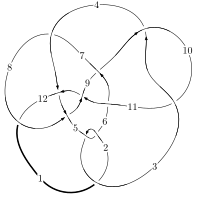
\includegraphics[width=112pt]{../../../GIT/diagram.site/Diagrams/png/2621_12n_0532.png}\\
\ \ \ A knot diagram\footnotemark}&
\allowdisplaybreaks
\textbf{Linearized knot diagam} \\
\cline{2-2}
 &
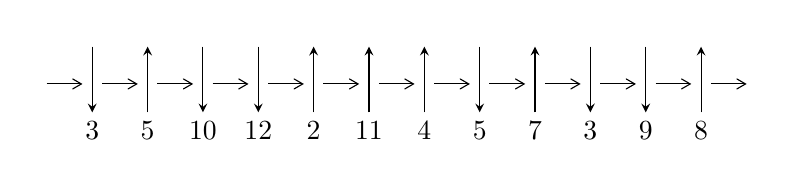
\begin{tikzpicture}[x=20pt, y=17pt]
	% nodes
	\node (C0) at (0, 0) {};
	\node (C1) at (1, 0) {};
	\node (C1U) at (1, +1) {};
	\node (C1D) at (1, -1) {3};

	\node (C2) at (2, 0) {};
	\node (C2U) at (2, +1) {};
	\node (C2D) at (2, -1) {5};

	\node (C3) at (3, 0) {};
	\node (C3U) at (3, +1) {};
	\node (C3D) at (3, -1) {10};

	\node (C4) at (4, 0) {};
	\node (C4U) at (4, +1) {};
	\node (C4D) at (4, -1) {12};

	\node (C5) at (5, 0) {};
	\node (C5U) at (5, +1) {};
	\node (C5D) at (5, -1) {2};

	\node (C6) at (6, 0) {};
	\node (C6U) at (6, +1) {};
	\node (C6D) at (6, -1) {11};

	\node (C7) at (7, 0) {};
	\node (C7U) at (7, +1) {};
	\node (C7D) at (7, -1) {4};

	\node (C8) at (8, 0) {};
	\node (C8U) at (8, +1) {};
	\node (C8D) at (8, -1) {5};

	\node (C9) at (9, 0) {};
	\node (C9U) at (9, +1) {};
	\node (C9D) at (9, -1) {7};

	\node (C10) at (10, 0) {};
	\node (C10U) at (10, +1) {};
	\node (C10D) at (10, -1) {3};

	\node (C11) at (11, 0) {};
	\node (C11U) at (11, +1) {};
	\node (C11D) at (11, -1) {9};

	\node (C12) at (12, 0) {};
	\node (C12U) at (12, +1) {};
	\node (C12D) at (12, -1) {8};
	\node (C13) at (13, 0) {};

	% arrows
	\draw[->,>={angle 60}]
	(C0) edge (C1) (C1) edge (C2) (C2) edge (C3) (C3) edge (C4) (C4) edge (C5) (C5) edge (C6) (C6) edge (C7) (C7) edge (C8) (C8) edge (C9) (C9) edge (C10) (C10) edge (C11) (C11) edge (C12) (C12) edge (C13) ;	\draw[->,>=stealth]
	(C1U) edge (C1D) (C2D) edge (C2U) (C3U) edge (C3D) (C4U) edge (C4D) (C5D) edge (C5U) (C6D) edge (C6U) (C7D) edge (C7U) (C8U) edge (C8D) (C9D) edge (C9U) (C10U) edge (C10D) (C11U) edge (C11D) (C12D) edge (C12U) ;
	\end{tikzpicture} \\
\hhline{~~} \\& 
\textbf{Solving Sequence} \\ \cline{2-2} 
 &
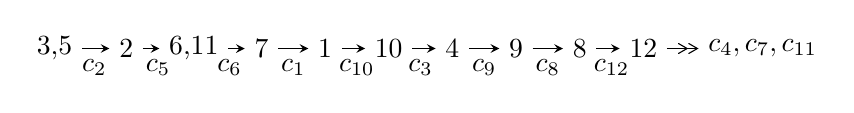
\begin{tikzpicture}[x=23pt, y=7pt]
	% node
	\node (A0) at (-1/8, 0) {3,5};
	\node (A1) at (1, 0) {2};
	\node (A2) at (33/16, 0) {6,11};
	\node (A3) at (25/8, 0) {7};
	\node (A4) at (33/8, 0) {1};
	\node (A5) at (41/8, 0) {10};
	\node (A6) at (49/8, 0) {4};
	\node (A7) at (57/8, 0) {9};
	\node (A8) at (65/8, 0) {8};
	\node (A9) at (73/8, 0) {12};
	\node (C1) at (1/2, -1) {$c_{2}$};
	\node (C2) at (3/2, -1) {$c_{5}$};
	\node (C3) at (21/8, -1) {$c_{6}$};
	\node (C4) at (29/8, -1) {$c_{1}$};
	\node (C5) at (37/8, -1) {$c_{10}$};
	\node (C6) at (45/8, -1) {$c_{3}$};
	\node (C7) at (53/8, -1) {$c_{9}$};
	\node (C8) at (61/8, -1) {$c_{8}$};
	\node (C9) at (69/8, -1) {$c_{12}$};
	\node (A10) at (11, 0) {$c_{4},c_{7},c_{11}$};

	% edge
	\draw[->,>=stealth]	
	(A0) edge (A1) (A1) edge (A2) (A2) edge (A3) (A3) edge (A4) (A4) edge (A5) (A5) edge (A6) (A6) edge (A7) (A7) edge (A8) (A8) edge (A9) ;
	\draw[->>,>={angle 60}]	
	(A9) edge (A10);
\end{tikzpicture} \\ 

\end{tabular} \\

\footnotetext{
The image of knot diagram is generated by the software ``\textbf{Draw programme}" developed by Andrew Bartholomew(\url{http://www.layer8.co.uk/maths/draw/index.htm\#Running-draw}), where we modified some parts for our purpose(\url{https://github.com/CATsTAILs/LinksPainter}).
}\phantom \\ \newline 
\centering \textbf{Ideals for irreducible components\footnotemark of $X_{\text{par}}$} 
 
\begin{align*}
I^u_{1}&=\langle 
-1.61870\times10^{329} u^{98}-5.11065\times10^{328} u^{97}+\cdots+4.51920\times10^{331} b-4.15006\times10^{331},\\
\phantom{I^u_{1}}&\phantom{= \langle  }3.15837\times10^{331} u^{98}-2.19273\times10^{330} u^{97}+\cdots+1.40095\times10^{333} a-5.59957\times10^{333},\\
\phantom{I^u_{1}}&\phantom{= \langle  }u^{99}+53 u^{97}+\cdots-259 u+31\rangle \\
I^u_{2}&=\langle 
-1.19415\times10^{16} u^{36}-1.97876\times10^{16} u^{35}+\cdots+3.72808\times10^{15} b+1.06100\times10^{16},\\
\phantom{I^u_{2}}&\phantom{= \langle  }-7.14844\times10^{15} u^{36}-9.64409\times10^{15} u^{35}+\cdots+3.72808\times10^{15} a-3.18284\times10^{16},\;u^{37}+u^{36}+\cdots-8 u-1\rangle \\
\\
\end{align*}
\raggedright * 2 irreducible components of $\dim_{\mathbb{C}}=0$, with total 136 representations.\\
\footnotetext{All coefficients of polynomials are rational numbers. But the coefficients are sometimes approximated in decimal forms when there is not enough margin.}
\newpage
\renewcommand{\arraystretch}{1}
\centering \section*{I. $I^u_{1}= \langle -1.62\times10^{329} u^{98}-5.11\times10^{328} u^{97}+\cdots+4.52\times10^{331} b-4.15\times10^{331},\;3.16\times10^{331} u^{98}-2.19\times10^{330} u^{97}+\cdots+1.40\times10^{333} a-5.60\times10^{333},\;u^{99}+53 u^{97}+\cdots-259 u+31 \rangle$}
\flushleft \textbf{(i) Arc colorings}\\
\begin{tabular}{m{7pt} m{180pt} m{7pt} m{180pt} }
\flushright $a_{3}=$&$\begin{pmatrix}1\\0\end{pmatrix}$ \\
\flushright $a_{5}=$&$\begin{pmatrix}0\\u\end{pmatrix}$ \\
\flushright $a_{2}=$&$\begin{pmatrix}1\\u^2\end{pmatrix}$ \\
\flushright $a_{6}=$&$\begin{pmatrix}u\\u^3+u\end{pmatrix}$ \\
\flushright $a_{11}=$&$\begin{pmatrix}-0.0225444 u^{98}+0.00156517 u^{97}+\cdots-98.9674 u+3.99697\\0.00358184 u^{98}+0.00113087 u^{97}+\cdots+0.568838 u+0.918316\end{pmatrix}$ \\
\flushright $a_{7}=$&$\begin{pmatrix}-0.0443461 u^{98}-0.00855901 u^{97}+\cdots-79.0333 u+1.08105\\0.00402845 u^{98}+0.000590727 u^{97}+\cdots-2.96656 u+0.894483\end{pmatrix}$ \\
\flushright $a_{1}=$&$\begin{pmatrix}u^2+1\\u^2\end{pmatrix}$ \\
\flushright $a_{10}=$&$\begin{pmatrix}-0.0189626 u^{98}+0.00269604 u^{97}+\cdots-98.3986 u+4.91529\\0.00358184 u^{98}+0.00113087 u^{97}+\cdots+0.568838 u+0.918316\end{pmatrix}$ \\
\flushright $a_{4}=$&$\begin{pmatrix}-0.0310245 u^{98}+0.00405756 u^{97}+\cdots-96.3241 u+6.72622\\-0.000256772 u^{98}-0.000349871 u^{97}+\cdots-3.51712 u+1.04145\end{pmatrix}$ \\
\flushright $a_{9}=$&$\begin{pmatrix}-0.0829098 u^{98}-0.00721519 u^{97}+\cdots-145.839 u-1.52124\\0.00219888 u^{98}+0.00435927 u^{97}+\cdots-14.5292 u+2.33219\end{pmatrix}$ \\
\flushright $a_{8}=$&$\begin{pmatrix}-0.0829098 u^{98}-0.00721519 u^{97}+\cdots-145.839 u-1.52124\\0.000152831 u^{98}+0.00273447 u^{97}+\cdots-15.2307 u+2.10852\end{pmatrix}$ \\
\flushright $a_{12}=$&$\begin{pmatrix}0.0180850 u^{98}-0.00679441 u^{97}+\cdots+40.9484 u-14.4549\\-0.00705979 u^{98}-0.00186554 u^{97}+\cdots-8.85440 u+0.261167\end{pmatrix}$\\&\end{tabular}
\flushleft \textbf{(ii) Obstruction class $= -1$}\\~\\
\flushleft \textbf{(iii) Cusp Shapes $= 0.0330848 u^{98}-0.00300896 u^{97}+\cdots+76.4947 u+7.16298$}\\~\\
\newpage\renewcommand{\arraystretch}{1}
\flushleft \textbf{(iv) u-Polynomials at the component}\newline \\
\begin{tabular}{m{50pt}|m{274pt}}
Crossings & \hspace{64pt}u-Polynomials at each crossing \\
\hline $$\begin{aligned}c_{1}\end{aligned}$$&$\begin{aligned}
&u^{99}+106 u^{98}+\cdots-170255 u-961
\end{aligned}$\\
\hline $$\begin{aligned}c_{2},c_{5}\end{aligned}$$&$\begin{aligned}
&u^{99}+53 u^{97}+\cdots-259 u+31
\end{aligned}$\\
\hline $$\begin{aligned}c_{3},c_{10}\end{aligned}$$&$\begin{aligned}
&u^{99}+27 u^{97}+\cdots-45156 u+28964
\end{aligned}$\\
\hline $$\begin{aligned}c_{4}\end{aligned}$$&$\begin{aligned}
&u^{99}+3 u^{98}+\cdots+29 u+1
\end{aligned}$\\
\hline $$\begin{aligned}c_{6}\end{aligned}$$&$\begin{aligned}
&u^{99}-8 u^{98}+\cdots+11559416 u+409289
\end{aligned}$\\
\hline $$\begin{aligned}c_{7}\end{aligned}$$&$\begin{aligned}
&u^{99}+u^{98}+\cdots+263227 u+47969
\end{aligned}$\\
\hline $$\begin{aligned}c_{8}\end{aligned}$$&$\begin{aligned}
&u^{99}+2 u^{98}+\cdots-5274 u-59
\end{aligned}$\\
\hline $$\begin{aligned}c_{9}\end{aligned}$$&$\begin{aligned}
&u^{99}-9 u^{98}+\cdots-402 u-215
\end{aligned}$\\
\hline $$\begin{aligned}c_{11}\end{aligned}$$&$\begin{aligned}
&u^{99}-6 u^{98}+\cdots-12984 u+3173
\end{aligned}$\\
\hline $$\begin{aligned}c_{12}\end{aligned}$$&$\begin{aligned}
&u^{99}- u^{98}+\cdots+11196996 u+1212452
\end{aligned}$\\
\hline
\end{tabular}\\~\\
\newpage\renewcommand{\arraystretch}{1}
\flushleft \textbf{(v) Riley Polynomials at the component}\newline \\
\begin{tabular}{m{50pt}|m{274pt}}
Crossings & \hspace{64pt}Riley Polynomials at each crossing \\
\hline $$\begin{aligned}c_{1}\end{aligned}$$&$\begin{aligned}
&y^{99}-198 y^{98}+\cdots-1536870623 y-923521
\end{aligned}$\\
\hline $$\begin{aligned}c_{2},c_{5}\end{aligned}$$&$\begin{aligned}
&y^{99}+106 y^{98}+\cdots-170255 y-961
\end{aligned}$\\
\hline $$\begin{aligned}c_{3},c_{10}\end{aligned}$$&$\begin{aligned}
&y^{99}+54 y^{98}+\cdots-26392577344 y-838913296
\end{aligned}$\\
\hline $$\begin{aligned}c_{4}\end{aligned}$$&$\begin{aligned}
&y^{99}+21 y^{98}+\cdots+287 y-1
\end{aligned}$\\
\hline $$\begin{aligned}c_{6}\end{aligned}$$&$\begin{aligned}
&y^{99}+14 y^{98}+\cdots+14727329603844 y-167517485521
\end{aligned}$\\
\hline $$\begin{aligned}c_{7}\end{aligned}$$&$\begin{aligned}
&y^{99}- y^{98}+\cdots+66159723473 y-2301024961
\end{aligned}$\\
\hline $$\begin{aligned}c_{8}\end{aligned}$$&$\begin{aligned}
&y^{99}-14 y^{98}+\cdots+8482664 y-3481
\end{aligned}$\\
\hline $$\begin{aligned}c_{9}\end{aligned}$$&$\begin{aligned}
&y^{99}-37 y^{98}+\cdots+769624 y-46225
\end{aligned}$\\
\hline $$\begin{aligned}c_{11}\end{aligned}$$&$\begin{aligned}
&y^{99}-20 y^{98}+\cdots-584095766 y-10067929
\end{aligned}$\\
\hline $$\begin{aligned}c_{12}\end{aligned}$$&$\begin{aligned}
&y^{99}+5 y^{98}+\cdots+5946396266144 y-1470039852304
\end{aligned}$\\
\hline
\end{tabular}\\~\\
\newpage\flushleft \textbf{(vi) Complex Volumes and Cusp Shapes}
$$\begin{array}{c|c|c}  
\text{Solutions to }I^u_{1}& \I (\text{vol} + \sqrt{-1}CS) & \text{Cusp shape}\\
 \hline 
\begin{aligned}
u &= -0.449463 + 0.920420 I \\
a &= \phantom{-}0.380654 - 0.863384 I \\
b &= -0.287498 - 1.090140 I\end{aligned}
 & \phantom{-}2.33708 - 5.55546 I & \phantom{-0.000000 } 0 \\ \hline\begin{aligned}
u &= -0.449463 - 0.920420 I \\
a &= \phantom{-}0.380654 + 0.863384 I \\
b &= -0.287498 + 1.090140 I\end{aligned}
 & \phantom{-}2.33708 + 5.55546 I & \phantom{-0.000000 } 0 \\ \hline\begin{aligned}
u &= \phantom{-}0.989702 + 0.361143 I \\
a &= \phantom{-}0.723225 + 0.816298 I \\
b &= -0.593040 + 1.230230 I\end{aligned}
 & \phantom{-}0.29355 + 4.78047 I & \phantom{-0.000000 } 0 \\ \hline\begin{aligned}
u &= \phantom{-}0.989702 - 0.361143 I \\
a &= \phantom{-}0.723225 - 0.816298 I \\
b &= -0.593040 - 1.230230 I\end{aligned}
 & \phantom{-}0.29355 - 4.78047 I & \phantom{-0.000000 } 0 \\ \hline\begin{aligned}
u &= \phantom{-}0.776838 + 0.723144 I \\
a &= \phantom{-}0.163427 + 0.003710 I \\
b &= \phantom{-}0.453158 + 0.898313 I\end{aligned}
 & -0.964664 + 0.845567 I & \phantom{-0.000000 } 0 \\ \hline\begin{aligned}
u &= \phantom{-}0.776838 - 0.723144 I \\
a &= \phantom{-}0.163427 - 0.003710 I \\
b &= \phantom{-}0.453158 - 0.898313 I\end{aligned}
 & -0.964664 - 0.845567 I & \phantom{-0.000000 } 0 \\ \hline\begin{aligned}
u &= -0.884203 + 0.198301 I \\
a &= -0.172383 + 1.092170 I \\
b &= \phantom{-}0.473016 + 0.798138 I\end{aligned}
 & -1.27586 - 4.76408 I & \phantom{-0.000000 } 0 \\ \hline\begin{aligned}
u &= -0.884203 - 0.198301 I \\
a &= -0.172383 - 1.092170 I \\
b &= \phantom{-}0.473016 - 0.798138 I\end{aligned}
 & -1.27586 + 4.76408 I & \phantom{-0.000000 } 0 \\ \hline\begin{aligned}
u &= -0.074327 + 1.099590 I \\
a &= \phantom{-}0.28126 + 2.12391 I \\
b &= -0.400780 - 0.695484 I\end{aligned}
 & \phantom{-}2.84341 + 2.27358 I & \phantom{-0.000000 } 0 \\ \hline\begin{aligned}
u &= -0.074327 - 1.099590 I \\
a &= \phantom{-}0.28126 - 2.12391 I \\
b &= -0.400780 + 0.695484 I\end{aligned}
 & \phantom{-}2.84341 - 2.27358 I & \phantom{-0.000000 } 0\\
 \hline 
 \end{array}$$\newpage$$\begin{array}{c|c|c}  
\text{Solutions to }I^u_{1}& \I (\text{vol} + \sqrt{-1}CS) & \text{Cusp shape}\\
 \hline 
\begin{aligned}
u &= \phantom{-}0.100382 + 1.131240 I \\
a &= \phantom{-}0.15482 + 2.33675 I \\
b &= \phantom{-}0.336290 - 0.620402 I\end{aligned}
 & \phantom{-}2.33767 + 5.94152 I & \phantom{-0.000000 } 0 \\ \hline\begin{aligned}
u &= \phantom{-}0.100382 - 1.131240 I \\
a &= \phantom{-}0.15482 - 2.33675 I \\
b &= \phantom{-}0.336290 + 0.620402 I\end{aligned}
 & \phantom{-}2.33767 - 5.94152 I & \phantom{-0.000000 } 0 \\ \hline\begin{aligned}
u &= \phantom{-}0.007624 + 0.863581 I \\
a &= -0.71439 + 1.52331 I \\
b &= \phantom{-}0.170924 - 1.193600 I\end{aligned}
 & \phantom{-}1.47026 + 4.79432 I & \phantom{-0.000000 } 0 \\ \hline\begin{aligned}
u &= \phantom{-}0.007624 - 0.863581 I \\
a &= -0.71439 - 1.52331 I \\
b &= \phantom{-}0.170924 + 1.193600 I\end{aligned}
 & \phantom{-}1.47026 - 4.79432 I & \phantom{-0.000000 } 0 \\ \hline\begin{aligned}
u &= \phantom{-}0.924315 + 0.669384 I \\
a &= \phantom{-}0.453346 + 0.855141 I \\
b &= -0.816396 + 0.665074 I\end{aligned}
 & -0.0948162 + 0.0797592 I & \phantom{-0.000000 } 0 \\ \hline\begin{aligned}
u &= \phantom{-}0.924315 - 0.669384 I \\
a &= \phantom{-}0.453346 - 0.855141 I \\
b &= -0.816396 - 0.665074 I\end{aligned}
 & -0.0948162 - 0.0797592 I & \phantom{-0.000000 } 0 \\ \hline\begin{aligned}
u &= -0.669840 + 0.535577 I \\
a &= \phantom{-}1.151360 - 0.720481 I \\
b &= \phantom{-}0.103338 - 0.884220 I\end{aligned}
 & \phantom{-}3.44466 + 1.11589 I & \phantom{-0.000000 } 0 \\ \hline\begin{aligned}
u &= -0.669840 - 0.535577 I \\
a &= \phantom{-}1.151360 + 0.720481 I \\
b &= \phantom{-}0.103338 + 0.884220 I\end{aligned}
 & \phantom{-}3.44466 - 1.11589 I & \phantom{-0.000000 } 0 \\ \hline\begin{aligned}
u &= \phantom{-}0.602702 + 0.978790 I \\
a &= -0.689533 + 0.399947 I \\
b &= -0.087589 - 0.819332 I\end{aligned}
 & \phantom{-}1.50660 + 3.93239 I & \phantom{-0.000000 } 0 \\ \hline\begin{aligned}
u &= \phantom{-}0.602702 - 0.978790 I \\
a &= -0.689533 - 0.399947 I \\
b &= -0.087589 + 0.819332 I\end{aligned}
 & \phantom{-}1.50660 - 3.93239 I & \phantom{-0.000000 } 0\\
 \hline 
 \end{array}$$\newpage$$\begin{array}{c|c|c}  
\text{Solutions to }I^u_{1}& \I (\text{vol} + \sqrt{-1}CS) & \text{Cusp shape}\\
 \hline 
\begin{aligned}
u &= \phantom{-}0.901703 + 0.736467 I \\
a &= -0.0451128 + 0.0657810 I \\
b &= \phantom{-}1.009140 + 0.461921 I\end{aligned}
 & -0.34961 + 6.23060 I & \phantom{-0.000000 } 0 \\ \hline\begin{aligned}
u &= \phantom{-}0.901703 - 0.736467 I \\
a &= -0.0451128 - 0.0657810 I \\
b &= \phantom{-}1.009140 - 0.461921 I\end{aligned}
 & -0.34961 - 6.23060 I & \phantom{-0.000000 } 0 \\ \hline\begin{aligned}
u &= \phantom{-}0.745265 + 0.362689 I \\
a &= \phantom{-}0.000194 - 0.396282 I \\
b &= \phantom{-}0.464260 - 0.826650 I\end{aligned}
 & \phantom{-}3.34931 + 1.03766 I & \phantom{-0.000000 } 0 \\ \hline\begin{aligned}
u &= \phantom{-}0.745265 - 0.362689 I \\
a &= \phantom{-}0.000194 + 0.396282 I \\
b &= \phantom{-}0.464260 + 0.826650 I\end{aligned}
 & \phantom{-}3.34931 - 1.03766 I & \phantom{-0.000000 } 0 \\ \hline\begin{aligned}
u &= \phantom{-}0.095723 + 0.821995 I \\
a &= \phantom{-}1.192920 + 0.548778 I \\
b &= \phantom{-}0.061204 - 1.279230 I\end{aligned}
 & \phantom{-}5.13444 + 0.35658 I & \phantom{-0.000000 } 0 \\ \hline\begin{aligned}
u &= \phantom{-}0.095723 - 0.821995 I \\
a &= \phantom{-}1.192920 - 0.548778 I \\
b &= \phantom{-}0.061204 + 1.279230 I\end{aligned}
 & \phantom{-}5.13444 - 0.35658 I & \phantom{-0.000000 } 0 \\ \hline\begin{aligned}
u &= -0.856107 + 0.834764 I \\
a &= \phantom{-}0.517321 - 0.351198 I \\
b &= -0.093212 - 0.986432 I\end{aligned}
 & \phantom{-}5.74308 - 3.12727 I & \phantom{-0.000000 } 0 \\ \hline\begin{aligned}
u &= -0.856107 - 0.834764 I \\
a &= \phantom{-}0.517321 + 0.351198 I \\
b &= -0.093212 + 0.986432 I\end{aligned}
 & \phantom{-}5.74308 + 3.12727 I & \phantom{-0.000000 } 0 \\ \hline\begin{aligned}
u &= \phantom{-}0.092174 + 0.789815 I \\
a &= -0.018180 + 0.859448 I \\
b &= \phantom{-}0.243265 - 1.352150 I\end{aligned}
 & \phantom{-}5.46584 + 4.99973 I & \phantom{-0.000000 } 0 \\ \hline\begin{aligned}
u &= \phantom{-}0.092174 - 0.789815 I \\
a &= -0.018180 - 0.859448 I \\
b &= \phantom{-}0.243265 + 1.352150 I\end{aligned}
 & \phantom{-}5.46584 - 4.99973 I & \phantom{-0.000000 } 0\\
 \hline 
 \end{array}$$\newpage$$\begin{array}{c|c|c}  
\text{Solutions to }I^u_{1}& \I (\text{vol} + \sqrt{-1}CS) & \text{Cusp shape}\\
 \hline 
\begin{aligned}
u &= -1.110540 + 0.511836 I \\
a &= -0.586814 + 0.687680 I \\
b &= \phantom{-}0.689492 + 1.188880 I\end{aligned}
 & \phantom{-}1.94491 - 12.39280 I & \phantom{-0.000000 } 0 \\ \hline\begin{aligned}
u &= -1.110540 - 0.511836 I \\
a &= -0.586814 - 0.687680 I \\
b &= \phantom{-}0.689492 - 1.188880 I\end{aligned}
 & \phantom{-}1.94491 + 12.39280 I & \phantom{-0.000000 } 0 \\ \hline\begin{aligned}
u &= -0.564604 + 0.483711 I \\
a &= \phantom{-}0.183144 - 0.072820 I \\
b &= -0.915705 + 0.256094 I\end{aligned}
 & -2.66072 + 0.68787 I & \phantom{-0.000000 } 0 \\ \hline\begin{aligned}
u &= -0.564604 - 0.483711 I \\
a &= \phantom{-}0.183144 + 0.072820 I \\
b &= -0.915705 - 0.256094 I\end{aligned}
 & -2.66072 - 0.68787 I & \phantom{-0.000000 } 0 \\ \hline\begin{aligned}
u &= \phantom{-}0.965432 + 0.809020 I \\
a &= -0.284876 - 0.157684 I \\
b &= \phantom{-}0.174022 - 0.782029 I\end{aligned}
 & \phantom{-}4.96132 + 3.43570 I & \phantom{-0.000000 } 0 \\ \hline\begin{aligned}
u &= \phantom{-}0.965432 - 0.809020 I \\
a &= -0.284876 + 0.157684 I \\
b &= \phantom{-}0.174022 + 0.782029 I\end{aligned}
 & \phantom{-}4.96132 - 3.43570 I & \phantom{-0.000000 } 0 \\ \hline\begin{aligned}
u &= -0.016021 + 0.727396 I \\
a &= \phantom{-}0.744128 + 0.572179 I \\
b &= -0.20015 - 1.40684 I\end{aligned}
 & \phantom{-}5.66046 - 4.73411 I & \phantom{-}7.47226 + 7.54887 I \\ \hline\begin{aligned}
u &= -0.016021 - 0.727396 I \\
a &= \phantom{-}0.744128 - 0.572179 I \\
b &= -0.20015 + 1.40684 I\end{aligned}
 & \phantom{-}5.66046 + 4.73411 I & \phantom{-}7.47226 - 7.54887 I \\ \hline\begin{aligned}
u &= -0.885265 + 0.922396 I \\
a &= \phantom{-}0.93169 - 1.63224 I \\
b &= -0.09307 - 1.62375 I\end{aligned}
 & \phantom{-}8.02930 - 3.25944 I & \phantom{-0.000000 } 0 \\ \hline\begin{aligned}
u &= -0.885265 - 0.922396 I \\
a &= \phantom{-}0.93169 + 1.63224 I \\
b &= -0.09307 + 1.62375 I\end{aligned}
 & \phantom{-}8.02930 + 3.25944 I & \phantom{-0.000000 } 0\\
 \hline 
 \end{array}$$\newpage$$\begin{array}{c|c|c}  
\text{Solutions to }I^u_{1}& \I (\text{vol} + \sqrt{-1}CS) & \text{Cusp shape}\\
 \hline 
\begin{aligned}
u &= -0.234061 + 0.612799 I \\
a &= \phantom{-}0.285773 - 0.530930 I \\
b &= -0.407982 - 1.268020 I\end{aligned}
 & \phantom{-}2.19138 - 5.42561 I & -2.53703 + 9.57555 I \\ \hline\begin{aligned}
u &= -0.234061 - 0.612799 I \\
a &= \phantom{-}0.285773 + 0.530930 I \\
b &= -0.407982 + 1.268020 I\end{aligned}
 & \phantom{-}2.19138 + 5.42561 I & -2.53703 - 9.57555 I \\ \hline\begin{aligned}
u &= -0.954291 + 0.953963 I \\
a &= -0.0892329 + 0.0111021 I \\
b &= -0.669835 + 0.942203 I\end{aligned}
 & \phantom{-}0.69700 + 5.44894 I & \phantom{-0.000000 } 0 \\ \hline\begin{aligned}
u &= -0.954291 - 0.953963 I \\
a &= -0.0892329 - 0.0111021 I \\
b &= -0.669835 - 0.942203 I\end{aligned}
 & \phantom{-}0.69700 - 5.44894 I & \phantom{-0.000000 } 0 \\ \hline\begin{aligned}
u &= \phantom{-}0.344285 + 0.509140 I \\
a &= \phantom{-}0.614615 + 0.516455 I \\
b &= -0.240304 + 0.507083 I\end{aligned}
 & -0.010371 + 1.152960 I & -0.45734 - 5.72489 I \\ \hline\begin{aligned}
u &= \phantom{-}0.344285 - 0.509140 I \\
a &= \phantom{-}0.614615 - 0.516455 I \\
b &= -0.240304 - 0.507083 I\end{aligned}
 & -0.010371 - 1.152960 I & -0.45734 + 5.72489 I \\ \hline\begin{aligned}
u &= \phantom{-}0.10854 + 1.45535 I \\
a &= \phantom{-}1.386540 + 0.042187 I \\
b &= -0.908690 + 0.807044 I\end{aligned}
 & -3.81992 - 0.72093 I & \phantom{-0.000000 } 0 \\ \hline\begin{aligned}
u &= \phantom{-}0.10854 - 1.45535 I \\
a &= \phantom{-}1.386540 - 0.042187 I \\
b &= -0.908690 - 0.807044 I\end{aligned}
 & -3.81992 + 0.72093 I & \phantom{-0.000000 } 0 \\ \hline\begin{aligned}
u &= -0.10960 + 1.46424 I \\
a &= -1.84124 + 0.02145 I \\
b &= \phantom{-}1.55189 + 0.62097 I\end{aligned}
 & -7.91560 - 1.49599 I & \phantom{-0.000000 } 0 \\ \hline\begin{aligned}
u &= -0.10960 - 1.46424 I \\
a &= -1.84124 - 0.02145 I \\
b &= \phantom{-}1.55189 - 0.62097 I\end{aligned}
 & -7.91560 + 1.49599 I & \phantom{-0.000000 } 0\\
 \hline 
 \end{array}$$\newpage$$\begin{array}{c|c|c}  
\text{Solutions to }I^u_{1}& \I (\text{vol} + \sqrt{-1}CS) & \text{Cusp shape}\\
 \hline 
\begin{aligned}
u &= -0.15530 + 1.47142 I \\
a &= -1.198180 + 0.213225 I \\
b &= \phantom{-}0.426419 + 0.517451 I\end{aligned}
 & -5.23087 + 1.77261 I & \phantom{-0.000000 } 0 \\ \hline\begin{aligned}
u &= -0.15530 - 1.47142 I \\
a &= -1.198180 - 0.213225 I \\
b &= \phantom{-}0.426419 - 0.517451 I\end{aligned}
 & -5.23087 - 1.77261 I & \phantom{-0.000000 } 0 \\ \hline\begin{aligned}
u &= -0.02559 + 1.47939 I \\
a &= \phantom{-}0.197837 - 0.543845 I \\
b &= -0.13512 + 1.81976 I\end{aligned}
 & -0.49001 - 3.57941 I & \phantom{-0.000000 } 0 \\ \hline\begin{aligned}
u &= -0.02559 - 1.47939 I \\
a &= \phantom{-}0.197837 + 0.543845 I \\
b &= -0.13512 - 1.81976 I\end{aligned}
 & -0.49001 + 3.57941 I & \phantom{-0.000000 } 0 \\ \hline\begin{aligned}
u &= \phantom{-}0.129823 + 0.501429 I \\
a &= \phantom{-}1.306120 + 0.239520 I \\
b &= -0.608170 + 0.458382 I\end{aligned}
 & -0.12758 + 2.03530 I & -3.94463 - 5.13845 I \\ \hline\begin{aligned}
u &= \phantom{-}0.129823 - 0.501429 I \\
a &= \phantom{-}1.306120 - 0.239520 I \\
b &= -0.608170 - 0.458382 I\end{aligned}
 & -0.12758 - 2.03530 I & -3.94463 + 5.13845 I \\ \hline\begin{aligned}
u &= \phantom{-}0.06552 + 1.50863 I \\
a &= \phantom{-}1.330260 + 0.045882 I \\
b &= -0.579457 + 1.015220 I\end{aligned}
 & -6.74620 - 1.98513 I & \phantom{-0.000000 } 0 \\ \hline\begin{aligned}
u &= \phantom{-}0.06552 - 1.50863 I \\
a &= \phantom{-}1.330260 - 0.045882 I \\
b &= -0.579457 - 1.015220 I\end{aligned}
 & -6.74620 + 1.98513 I & \phantom{-0.000000 } 0 \\ \hline\begin{aligned}
u &= \phantom{-}0.15031 + 1.50678 I \\
a &= \phantom{-}1.335870 - 0.314116 I \\
b &= -1.06177 + 1.05023 I\end{aligned}
 & -2.85225 + 3.92690 I & \phantom{-0.000000 } 0 \\ \hline\begin{aligned}
u &= \phantom{-}0.15031 - 1.50678 I \\
a &= \phantom{-}1.335870 + 0.314116 I \\
b &= -1.06177 - 1.05023 I\end{aligned}
 & -2.85225 - 3.92690 I & \phantom{-0.000000 } 0\\
 \hline 
 \end{array}$$\newpage$$\begin{array}{c|c|c}  
\text{Solutions to }I^u_{1}& \I (\text{vol} + \sqrt{-1}CS) & \text{Cusp shape}\\
 \hline 
\begin{aligned}
u &= \phantom{-}0.29344 + 1.51721 I \\
a &= -1.293750 - 0.102136 I \\
b &= \phantom{-}0.656632 - 1.048550 I\end{aligned}
 & -7.22483 + 4.07577 I & \phantom{-0.000000 } 0 \\ \hline\begin{aligned}
u &= \phantom{-}0.29344 - 1.51721 I \\
a &= -1.293750 + 0.102136 I \\
b &= \phantom{-}0.656632 + 1.048550 I\end{aligned}
 & -7.22483 - 4.07577 I & \phantom{-0.000000 } 0 \\ \hline\begin{aligned}
u &= \phantom{-}0.09950 + 1.54213 I \\
a &= -1.44627 + 0.26452 I \\
b &= \phantom{-}0.854251 - 0.847301 I\end{aligned}
 & -6.87766 + 3.21394 I & \phantom{-0.000000 } 0 \\ \hline\begin{aligned}
u &= \phantom{-}0.09950 - 1.54213 I \\
a &= -1.44627 - 0.26452 I \\
b &= \phantom{-}0.854251 + 0.847301 I\end{aligned}
 & -6.87766 - 3.21394 I & \phantom{-0.000000 } 0 \\ \hline\begin{aligned}
u &= -0.42150 + 1.49357 I \\
a &= \phantom{-}1.153460 - 0.212027 I \\
b &= -0.562638 - 1.165240 I\end{aligned}
 & -6.71949 - 9.70184 I & \phantom{-0.000000 } 0 \\ \hline\begin{aligned}
u &= -0.42150 - 1.49357 I \\
a &= \phantom{-}1.153460 + 0.212027 I \\
b &= -0.562638 + 1.165240 I\end{aligned}
 & -6.71949 + 9.70184 I & \phantom{-0.000000 } 0 \\ \hline\begin{aligned}
u &= -0.09642 + 1.55493 I \\
a &= -1.249440 - 0.615146 I \\
b &= \phantom{-}0.88571 + 1.37991 I\end{aligned}
 & -5.07786 - 6.90046 I & \phantom{-0.000000 } 0 \\ \hline\begin{aligned}
u &= -0.09642 - 1.55493 I \\
a &= -1.249440 + 0.615146 I \\
b &= \phantom{-}0.88571 - 1.37991 I\end{aligned}
 & -5.07786 + 6.90046 I & \phantom{-0.000000 } 0 \\ \hline\begin{aligned}
u &= \phantom{-}0.01774 + 1.58324 I \\
a &= -0.569305 + 0.524028 I \\
b &= \phantom{-}0.18170 + 1.41637 I\end{aligned}
 & -2.16703 - 4.61474 I & \phantom{-0.000000 } 0 \\ \hline\begin{aligned}
u &= \phantom{-}0.01774 - 1.58324 I \\
a &= -0.569305 - 0.524028 I \\
b &= \phantom{-}0.18170 - 1.41637 I\end{aligned}
 & -2.16703 + 4.61474 I & \phantom{-0.000000 } 0\\
 \hline 
 \end{array}$$\newpage$$\begin{array}{c|c|c}  
\text{Solutions to }I^u_{1}& \I (\text{vol} + \sqrt{-1}CS) & \text{Cusp shape}\\
 \hline 
\begin{aligned}
u &= -0.11523 + 1.58503 I \\
a &= -1.258050 - 0.232343 I \\
b &= \phantom{-}0.344246 + 0.941272 I\end{aligned}
 & -3.94420 - 1.39890 I & \phantom{-0.000000 } 0 \\ \hline\begin{aligned}
u &= -0.11523 - 1.58503 I \\
a &= -1.258050 + 0.232343 I \\
b &= \phantom{-}0.344246 - 0.941272 I\end{aligned}
 & -3.94420 + 1.39890 I & \phantom{-0.000000 } 0 \\ \hline\begin{aligned}
u &= -0.26660 + 1.56711 I \\
a &= -1.225090 + 0.523394 I \\
b &= \phantom{-}1.39876 - 0.31492 I\end{aligned}
 & -9.32625 - 2.79394 I & \phantom{-0.000000 } 0 \\ \hline\begin{aligned}
u &= -0.26660 - 1.56711 I \\
a &= -1.225090 - 0.523394 I \\
b &= \phantom{-}1.39876 + 0.31492 I\end{aligned}
 & -9.32625 + 2.79394 I & \phantom{-0.000000 } 0 \\ \hline\begin{aligned}
u &= \phantom{-}0.16827 + 1.59853 I \\
a &= \phantom{-}1.106590 - 0.431611 I \\
b &= -0.805158 + 0.968421 I\end{aligned}
 & -3.29792 + 7.02458 I & \phantom{-0.000000 } 0 \\ \hline\begin{aligned}
u &= \phantom{-}0.16827 - 1.59853 I \\
a &= \phantom{-}1.106590 + 0.431611 I \\
b &= -0.805158 - 0.968421 I\end{aligned}
 & -3.29792 - 7.02458 I & \phantom{-0.000000 } 0 \\ \hline\begin{aligned}
u &= \phantom{-}0.42078 + 1.55266 I \\
a &= -1.50413 - 0.03210 I \\
b &= \phantom{-}0.71068 - 1.37025 I\end{aligned}
 & -5.84524 + 10.03770 I & \phantom{-0.000000 } 0 \\ \hline\begin{aligned}
u &= \phantom{-}0.42078 - 1.55266 I \\
a &= -1.50413 + 0.03210 I \\
b &= \phantom{-}0.71068 + 1.37025 I\end{aligned}
 & -5.84524 - 10.03770 I & \phantom{-0.000000 } 0 \\ \hline\begin{aligned}
u &= \phantom{-}0.122026 + 0.366129 I \\
a &= \phantom{-}3.37423 - 4.46100 I \\
b &= -0.291352 - 1.174280 I\end{aligned}
 & \phantom{-}4.86450 - 5.17783 I & \phantom{-}9.36120 + 6.43156 I \\ \hline\begin{aligned}
u &= \phantom{-}0.122026 - 0.366129 I \\
a &= \phantom{-}3.37423 + 4.46100 I \\
b &= -0.291352 + 1.174280 I\end{aligned}
 & \phantom{-}4.86450 + 5.17783 I & \phantom{-}9.36120 - 6.43156 I\\
 \hline 
 \end{array}$$\newpage$$\begin{array}{c|c|c}  
\text{Solutions to }I^u_{1}& \I (\text{vol} + \sqrt{-1}CS) & \text{Cusp shape}\\
 \hline 
\begin{aligned}
u &= -0.11601 + 1.61062 I \\
a &= -1.092310 - 0.514662 I \\
b &= \phantom{-}0.554317 + 1.164830 I\end{aligned}
 & -2.89782 - 5.94500 I & \phantom{-0.000000 } 0 \\ \hline\begin{aligned}
u &= -0.11601 - 1.61062 I \\
a &= -1.092310 + 0.514662 I \\
b &= \phantom{-}0.554317 - 1.164830 I\end{aligned}
 & -2.89782 + 5.94500 I & \phantom{-0.000000 } 0 \\ \hline\begin{aligned}
u &= \phantom{-}0.24750 + 1.63553 I \\
a &= \phantom{-}1.205180 + 0.393283 I \\
b &= -1.41575 - 0.32390 I\end{aligned}
 & -8.31396 + 10.41990 I & \phantom{-0.000000 } 0 \\ \hline\begin{aligned}
u &= \phantom{-}0.24750 - 1.63553 I \\
a &= \phantom{-}1.205180 - 0.393283 I \\
b &= -1.41575 + 0.32390 I\end{aligned}
 & -8.31396 - 10.41990 I & \phantom{-0.000000 } 0 \\ \hline\begin{aligned}
u &= \phantom{-}0.10452 + 1.65273 I \\
a &= \phantom{-}1.115920 - 0.696101 I \\
b &= -0.413837 + 0.798020 I\end{aligned}
 & -7.63047 + 6.05503 I & \phantom{-0.000000 } 0 \\ \hline\begin{aligned}
u &= \phantom{-}0.10452 - 1.65273 I \\
a &= \phantom{-}1.115920 + 0.696101 I \\
b &= -0.413837 - 0.798020 I\end{aligned}
 & -7.63047 - 6.05503 I & \phantom{-0.000000 } 0 \\ \hline\begin{aligned}
u &= -0.40356 + 1.60685 I \\
a &= \phantom{-}1.411000 + 0.036399 I \\
b &= -0.75772 - 1.38230 I\end{aligned}
 & -4.8993 - 17.9291 I & \phantom{-0.000000 } 0 \\ \hline\begin{aligned}
u &= -0.40356 - 1.60685 I \\
a &= \phantom{-}1.411000 - 0.036399 I \\
b &= -0.75772 + 1.38230 I\end{aligned}
 & -4.8993 + 17.9291 I & \phantom{-0.000000 } 0 \\ \hline\begin{aligned}
u &= \phantom{-}0.22703 + 1.66260 I \\
a &= \phantom{-}0.668359 + 0.230859 I \\
b &= -0.692357 - 0.412144 I\end{aligned}
 & -9.05435 + 4.80057 I & \phantom{-0.000000 } 0 \\ \hline\begin{aligned}
u &= \phantom{-}0.22703 - 1.66260 I \\
a &= \phantom{-}0.668359 - 0.230859 I \\
b &= -0.692357 + 0.412144 I\end{aligned}
 & -9.05435 - 4.80057 I & \phantom{-0.000000 } 0\\
 \hline 
 \end{array}$$\newpage$$\begin{array}{c|c|c}  
\text{Solutions to }I^u_{1}& \I (\text{vol} + \sqrt{-1}CS) & \text{Cusp shape}\\
 \hline 
\begin{aligned}
u &= -0.15035 + 1.67413 I \\
a &= -0.841817 + 0.262191 I \\
b &= \phantom{-}0.866086 - 0.528143 I\end{aligned}
 & -8.78633 + 1.54908 I & \phantom{-0.000000 } 0 \\ \hline\begin{aligned}
u &= -0.15035 - 1.67413 I \\
a &= -0.841817 - 0.262191 I \\
b &= \phantom{-}0.866086 + 0.528143 I\end{aligned}
 & -8.78633 - 1.54908 I & \phantom{-0.000000 } 0 \\ \hline\begin{aligned}
u &= -0.129576 + 0.278011 I \\
a &= -2.76297 - 3.97519 I \\
b &= \phantom{-}0.273923 - 1.343870 I\end{aligned}
 & \phantom{-}5.51201 - 2.99398 I & \phantom{-}8.78954 + 4.65677 I \\ \hline\begin{aligned}
u &= -0.129576 - 0.278011 I \\
a &= -2.76297 + 3.97519 I \\
b &= \phantom{-}0.273923 + 1.343870 I\end{aligned}
 & \phantom{-}5.51201 + 2.99398 I & \phantom{-}8.78954 - 4.65677 I \\ \hline\begin{aligned}
u &= -0.303524\phantom{ +0.000000I} \\
a &= -1.02169\phantom{ +0.000000I} \\
b &= -1.39193\phantom{ +0.000000I}\end{aligned}
 & -2.63515\phantom{ +0.000000I} & -38.4420\phantom{ +0.000000I} \\ \hline\begin{aligned}
u &= \phantom{-}0.091053 + 0.167445 I \\
a &= -3.33529 - 6.24003 I \\
b &= \phantom{-}0.244481 - 0.486448 I\end{aligned}
 & -0.77407 - 2.77339 I & -4.75332 - 5.97266 I \\ \hline\begin{aligned}
u &= \phantom{-}0.091053 - 0.167445 I \\
a &= -3.33529 + 6.24003 I \\
b &= \phantom{-}0.244481 + 0.486448 I\end{aligned}
 & -0.77407 + 2.77339 I & -4.75332 + 5.97266 I \\ \hline\begin{aligned}
u &= \phantom{-}0.0480242 + 0.1073590 I \\
a &= -0.96262 - 6.51872 I \\
b &= \phantom{-}0.606334 - 0.040916 I\end{aligned}
 & \phantom{-}1.33337 - 1.63871 I & \phantom{-}3.10567 + 5.35613 I \\ \hline\begin{aligned}
u &= \phantom{-}0.0480242 - 0.1073590 I \\
a &= -0.96262 + 6.51872 I \\
b &= \phantom{-}0.606334 + 0.040916 I\end{aligned}
 & \phantom{-}1.33337 + 1.63871 I & \phantom{-}3.10567 - 5.35613 I\\
 \hline 
 \end{array}$$\newpage\newpage\renewcommand{\arraystretch}{1}
\centering \section*{II. $I^u_{2}= \langle -1.19\times10^{16} u^{36}-1.98\times10^{16} u^{35}+\cdots+3.73\times10^{15} b+1.06\times10^{16},\;-7.15\times10^{15} u^{36}-9.64\times10^{15} u^{35}+\cdots+3.73\times10^{15} a-3.18\times10^{16},\;u^{37}+u^{36}+\cdots-8 u-1 \rangle$}
\flushleft \textbf{(i) Arc colorings}\\
\begin{tabular}{m{7pt} m{180pt} m{7pt} m{180pt} }
\flushright $a_{3}=$&$\begin{pmatrix}1\\0\end{pmatrix}$ \\
\flushright $a_{5}=$&$\begin{pmatrix}0\\u\end{pmatrix}$ \\
\flushright $a_{2}=$&$\begin{pmatrix}1\\u^2\end{pmatrix}$ \\
\flushright $a_{6}=$&$\begin{pmatrix}u\\u^3+u\end{pmatrix}$ \\
\flushright $a_{11}=$&$\begin{pmatrix}1.91746 u^{36}+2.58688 u^{35}+\cdots+33.7288 u+8.53747\\3.20312 u^{36}+5.30772 u^{35}+\cdots-24.5888 u-2.84598\end{pmatrix}$ \\
\flushright $a_{7}=$&$\begin{pmatrix}1.04256 u^{36}+4.09694 u^{35}+\cdots-55.3349 u-11.7400\\-1.90326 u^{36}-1.85536 u^{35}+\cdots+12.3168 u+1.70320\end{pmatrix}$ \\
\flushright $a_{1}=$&$\begin{pmatrix}u^2+1\\u^2\end{pmatrix}$ \\
\flushright $a_{10}=$&$\begin{pmatrix}5.12058 u^{36}+7.89460 u^{35}+\cdots+9.14006 u+5.69149\\3.20312 u^{36}+5.30772 u^{35}+\cdots-24.5888 u-2.84598\end{pmatrix}$ \\
\flushright $a_{4}=$&$\begin{pmatrix}-0.266371 u^{36}-5.46191 u^{35}+\cdots-10.7557 u+0.388655\\-2.36436 u^{36}-2.41065 u^{35}+\cdots+1.03658 u-1.72594\end{pmatrix}$ \\
\flushright $a_{9}=$&$\begin{pmatrix}-0.200511 u^{36}-0.943207 u^{35}+\cdots+41.2246 u+2.53862\\-1.71820 u^{36}-4.55410 u^{35}+\cdots+18.6360 u+3.32754\end{pmatrix}$ \\
\flushright $a_{8}=$&$\begin{pmatrix}-0.200511 u^{36}-0.943207 u^{35}+\cdots+41.2246 u+2.53862\\-0.572081 u^{36}-4.05875 u^{35}+\cdots+24.7780 u+4.07023\end{pmatrix}$ \\
\flushright $a_{12}=$&$\begin{pmatrix}-0.121535 u^{36}+0.541641 u^{35}+\cdots+53.1666 u+7.56314\\-0.669721 u^{36}-2.37534 u^{35}+\cdots-2.31374 u+0.533701\end{pmatrix}$\\&\end{tabular}
\flushleft \textbf{(ii) Obstruction class $= 1$}\\~\\
\flushleft \textbf{(iii) Cusp Shapes $= -\frac{37923239655330084}{3728078412487259} u^{36}-\frac{38434343438741474}{3728078412487259} u^{35}+\cdots+\frac{122400492787805403}{3728078412487259} u+\frac{30710588913013107}{3728078412487259}$}\\~\\
\newpage\renewcommand{\arraystretch}{1}
\flushleft \textbf{(iv) u-Polynomials at the component}\newline \\
\begin{tabular}{m{50pt}|m{274pt}}
Crossings & \hspace{64pt}u-Polynomials at each crossing \\
\hline $$\begin{aligned}c_{1}\end{aligned}$$&$\begin{aligned}
&u^{37}-37 u^{36}+\cdots-12 u+1
\end{aligned}$\\
\hline $$\begin{aligned}c_{2}\end{aligned}$$&$\begin{aligned}
&u^{37}+u^{36}+\cdots-8 u-1
\end{aligned}$\\
\hline $$\begin{aligned}c_{3}\end{aligned}$$&$\begin{aligned}
&u^{37}- u^{36}+\cdots-6 u+4
\end{aligned}$\\
\hline $$\begin{aligned}c_{4}\end{aligned}$$&$\begin{aligned}
&u^{37}-2 u^{36}+\cdots+u^2+1
\end{aligned}$\\
\hline $$\begin{aligned}c_{5}\end{aligned}$$&$\begin{aligned}
&u^{37}- u^{36}+\cdots-8 u+1
\end{aligned}$\\
\hline $$\begin{aligned}c_{6}\end{aligned}$$&$\begin{aligned}
&u^{37}-7 u^{36}+\cdots-253 u+41
\end{aligned}$\\
\hline $$\begin{aligned}c_{7}\end{aligned}$$&$\begin{aligned}
&u^{37}+2 u^{36}+\cdots-224 u-23
\end{aligned}$\\
\hline $$\begin{aligned}c_{8}\end{aligned}$$&$\begin{aligned}
&u^{37}- u^{36}+\cdots+3 u+1
\end{aligned}$\\
\hline $$\begin{aligned}c_{9}\end{aligned}$$&$\begin{aligned}
&u^{37}-18 u^{36}+\cdots+15 u-1
\end{aligned}$\\
\hline $$\begin{aligned}c_{10}\end{aligned}$$&$\begin{aligned}
&u^{37}+u^{36}+\cdots-6 u-4
\end{aligned}$\\
\hline $$\begin{aligned}c_{11}\end{aligned}$$&$\begin{aligned}
&u^{37}+3 u^{36}+\cdots-7 u+1
\end{aligned}$\\
\hline $$\begin{aligned}c_{12}\end{aligned}$$&$\begin{aligned}
&u^{37}-10 u^{35}+\cdots-12 u+4
\end{aligned}$\\
\hline
\end{tabular}\\~\\
\newpage\renewcommand{\arraystretch}{1}
\flushleft \textbf{(v) Riley Polynomials at the component}\newline \\
\begin{tabular}{m{50pt}|m{274pt}}
Crossings & \hspace{64pt}Riley Polynomials at each crossing \\
\hline $$\begin{aligned}c_{1}\end{aligned}$$&$\begin{aligned}
&y^{37}-47 y^{36}+\cdots-1240 y-1
\end{aligned}$\\
\hline $$\begin{aligned}c_{2},c_{5}\end{aligned}$$&$\begin{aligned}
&y^{37}+37 y^{36}+\cdots-12 y-1
\end{aligned}$\\
\hline $$\begin{aligned}c_{3},c_{10}\end{aligned}$$&$\begin{aligned}
&y^{37}+29 y^{36}+\cdots-164 y-16
\end{aligned}$\\
\hline $$\begin{aligned}c_{4}\end{aligned}$$&$\begin{aligned}
&y^{37}+12 y^{36}+\cdots-2 y-1
\end{aligned}$\\
\hline $$\begin{aligned}c_{6}\end{aligned}$$&$\begin{aligned}
&y^{37}-27 y^{36}+\cdots-148617 y-1681
\end{aligned}$\\
\hline $$\begin{aligned}c_{7}\end{aligned}$$&$\begin{aligned}
&y^{37}-2 y^{36}+\cdots+28740 y-529
\end{aligned}$\\
\hline $$\begin{aligned}c_{8}\end{aligned}$$&$\begin{aligned}
&y^{37}+17 y^{36}+\cdots-5 y-1
\end{aligned}$\\
\hline $$\begin{aligned}c_{9}\end{aligned}$$&$\begin{aligned}
&y^{37}-18 y^{36}+\cdots+15 y-1
\end{aligned}$\\
\hline $$\begin{aligned}c_{11}\end{aligned}$$&$\begin{aligned}
&y^{37}- y^{36}+\cdots+37 y-1
\end{aligned}$\\
\hline $$\begin{aligned}c_{12}\end{aligned}$$&$\begin{aligned}
&y^{37}-20 y^{36}+\cdots+248 y-16
\end{aligned}$\\
\hline
\end{tabular}\\~\\
\newpage\flushleft \textbf{(vi) Complex Volumes and Cusp Shapes}
$$\begin{array}{c|c|c}  
\text{Solutions to }I^u_{2}& \I (\text{vol} + \sqrt{-1}CS) & \text{Cusp shape}\\
 \hline 
\begin{aligned}
u &= \phantom{-}0.338592 + 0.948860 I \\
a &= \phantom{-}0.95168 - 1.83322 I \\
b &= \phantom{-}0.265936 + 0.997961 I\end{aligned}
 & \phantom{-}3.86482 - 4.14135 I & \phantom{-}4.53105 + 3.04755 I \\ \hline\begin{aligned}
u &= \phantom{-}0.338592 - 0.948860 I \\
a &= \phantom{-}0.95168 + 1.83322 I \\
b &= \phantom{-}0.265936 - 0.997961 I\end{aligned}
 & \phantom{-}3.86482 + 4.14135 I & \phantom{-}4.53105 - 3.04755 I \\ \hline\begin{aligned}
u &= \phantom{-}0.265057 + 0.991414 I \\
a &= \phantom{-}0.14714 + 2.27315 I \\
b &= -0.238262 + 1.085470 I\end{aligned}
 & \phantom{-}3.72363 + 6.48494 I & \phantom{-}5.58596 - 8.59239 I \\ \hline\begin{aligned}
u &= \phantom{-}0.265057 - 0.991414 I \\
a &= \phantom{-}0.14714 - 2.27315 I \\
b &= -0.238262 - 1.085470 I\end{aligned}
 & \phantom{-}3.72363 - 6.48494 I & \phantom{-}5.58596 + 8.59239 I \\ \hline\begin{aligned}
u &= \phantom{-}0.231695 + 1.053600 I \\
a &= -0.328847 + 0.338447 I \\
b &= \phantom{-}0.13679 - 1.41355 I\end{aligned}
 & \phantom{-}5.02855 + 5.83791 I & \phantom{-}2.12557 - 10.81625 I \\ \hline\begin{aligned}
u &= \phantom{-}0.231695 - 1.053600 I \\
a &= -0.328847 - 0.338447 I \\
b &= \phantom{-}0.13679 + 1.41355 I\end{aligned}
 & \phantom{-}5.02855 - 5.83791 I & \phantom{-}2.12557 + 10.81625 I \\ \hline\begin{aligned}
u &= -0.504429 + 0.758589 I \\
a &= \phantom{-}0.559317 - 1.148640 I \\
b &= -0.737197 - 0.134602 I\end{aligned}
 & \phantom{-}1.270810 + 0.262848 I & \phantom{-}2.31162 - 0.46763 I \\ \hline\begin{aligned}
u &= -0.504429 - 0.758589 I \\
a &= \phantom{-}0.559317 + 1.148640 I \\
b &= -0.737197 + 0.134602 I\end{aligned}
 & \phantom{-}1.270810 - 0.262848 I & \phantom{-}2.31162 + 0.46763 I \\ \hline\begin{aligned}
u &= \phantom{-}0.249444 + 0.875212 I \\
a &= -0.021257 + 0.483417 I \\
b &= -0.27473 - 1.39700 I\end{aligned}
 & \phantom{-}5.68845 - 3.92908 I & \phantom{-}6.71923 - 2.63498 I \\ \hline\begin{aligned}
u &= \phantom{-}0.249444 - 0.875212 I \\
a &= -0.021257 - 0.483417 I \\
b &= -0.27473 + 1.39700 I\end{aligned}
 & \phantom{-}5.68845 + 3.92908 I & \phantom{-}6.71923 + 2.63498 I\\
 \hline 
 \end{array}$$\newpage$$\begin{array}{c|c|c}  
\text{Solutions to }I^u_{2}& \I (\text{vol} + \sqrt{-1}CS) & \text{Cusp shape}\\
 \hline 
\begin{aligned}
u &= -0.500516 + 1.000950 I \\
a &= \phantom{-}0.062067 - 0.430630 I \\
b &= \phantom{-}0.337894 - 0.143349 I\end{aligned}
 & \phantom{-}0.32441 - 4.22499 I & -2.12351 + 6.06500 I \\ \hline\begin{aligned}
u &= -0.500516 - 1.000950 I \\
a &= \phantom{-}0.062067 + 0.430630 I \\
b &= \phantom{-}0.337894 + 0.143349 I\end{aligned}
 & \phantom{-}0.32441 + 4.22499 I & -2.12351 - 6.06500 I \\ \hline\begin{aligned}
u &= -0.244376 + 1.096530 I \\
a &= -0.27055 - 1.92483 I \\
b &= -0.323355 + 1.155810 I\end{aligned}
 & \phantom{-}3.72196 - 3.98898 I & \phantom{-}5.38613 + 4.17982 I \\ \hline\begin{aligned}
u &= -0.244376 - 1.096530 I \\
a &= -0.27055 + 1.92483 I \\
b &= -0.323355 - 1.155810 I\end{aligned}
 & \phantom{-}3.72196 + 3.98898 I & \phantom{-}5.38613 - 4.17982 I \\ \hline\begin{aligned}
u &= -0.242362 + 0.837304 I \\
a &= \phantom{-}0.55946 + 1.62396 I \\
b &= \phantom{-}0.190027 + 1.190510 I\end{aligned}
 & \phantom{-}4.70330 + 2.04272 I & \phantom{-}4.49829 - 0.65248 I \\ \hline\begin{aligned}
u &= -0.242362 - 0.837304 I \\
a &= \phantom{-}0.55946 - 1.62396 I \\
b &= \phantom{-}0.190027 - 1.190510 I\end{aligned}
 & \phantom{-}4.70330 - 2.04272 I & \phantom{-}4.49829 + 0.65248 I \\ \hline\begin{aligned}
u &= \phantom{-}0.645588 + 0.949229 I \\
a &= -0.342734 + 0.071468 I \\
b &= -0.077111 - 1.181410 I\end{aligned}
 & \phantom{-}6.43211 + 2.47921 I & \phantom{-}10.05169 + 1.00369 I \\ \hline\begin{aligned}
u &= \phantom{-}0.645588 - 0.949229 I \\
a &= -0.342734 - 0.071468 I \\
b &= -0.077111 + 1.181410 I\end{aligned}
 & \phantom{-}6.43211 - 2.47921 I & \phantom{-}10.05169 - 1.00369 I \\ \hline\begin{aligned}
u &= -0.946846 + 0.848293 I \\
a &= \phantom{-}0.291766 - 0.264862 I \\
b &= -0.156013 - 0.757712 I\end{aligned}
 & \phantom{-}4.74806 - 3.40411 I & -13.02147 + 0. I\phantom{ +0.000000I} \\ \hline\begin{aligned}
u &= -0.946846 - 0.848293 I \\
a &= \phantom{-}0.291766 + 0.264862 I \\
b &= -0.156013 + 0.757712 I\end{aligned}
 & \phantom{-}4.74806 + 3.40411 I & -13.02147 + 0. I\phantom{ +0.000000I}\\
 \hline 
 \end{array}$$\newpage$$\begin{array}{c|c|c}  
\text{Solutions to }I^u_{2}& \I (\text{vol} + \sqrt{-1}CS) & \text{Cusp shape}\\
 \hline 
\begin{aligned}
u &= \phantom{-}0.860354 + 0.946621 I \\
a &= \phantom{-}1.02362 + 1.62425 I \\
b &= -0.11292 + 1.61129 I\end{aligned}
 & \phantom{-}8.07656 + 3.17381 I & \phantom{-}22.1999 + 33.1535 I \\ \hline\begin{aligned}
u &= \phantom{-}0.860354 - 0.946621 I \\
a &= \phantom{-}1.02362 - 1.62425 I \\
b &= -0.11292 - 1.61129 I\end{aligned}
 & \phantom{-}8.07656 - 3.17381 I & \phantom{-}22.1999 - 33.1535 I \\ \hline\begin{aligned}
u &= -0.14840 + 1.48072 I \\
a &= -1.283810 + 0.166064 I \\
b &= \phantom{-}0.596153 + 0.750938 I\end{aligned}
 & -5.26789 + 1.08040 I & \phantom{-0.000000 } 0 \\ \hline\begin{aligned}
u &= -0.14840 - 1.48072 I \\
a &= -1.283810 - 0.166064 I \\
b &= \phantom{-}0.596153 - 0.750938 I\end{aligned}
 & -5.26789 - 1.08040 I & \phantom{-0.000000 } 0 \\ \hline\begin{aligned}
u &= \phantom{-}0.13422 + 1.49054 I \\
a &= -1.70068 - 0.10708 I \\
b &= \phantom{-}1.44159 - 0.39456 I\end{aligned}
 & -7.97369 + 1.95650 I & \phantom{-0.000000 } 0 \\ \hline\begin{aligned}
u &= \phantom{-}0.13422 - 1.49054 I \\
a &= -1.70068 + 0.10708 I \\
b &= \phantom{-}1.44159 + 0.39456 I\end{aligned}
 & -7.97369 - 1.95650 I & \phantom{-0.000000 } 0 \\ \hline\begin{aligned}
u &= -0.402019 + 0.253719 I \\
a &= -2.24388 + 1.02418 I \\
b &= -0.097540 + 0.470442 I\end{aligned}
 & -0.59112 - 3.13623 I & \phantom{-}3.97798 + 11.06924 I \\ \hline\begin{aligned}
u &= -0.402019 - 0.253719 I \\
a &= -2.24388 - 1.02418 I \\
b &= -0.097540 - 0.470442 I\end{aligned}
 & -0.59112 + 3.13623 I & \phantom{-}3.97798 - 11.06924 I \\ \hline\begin{aligned}
u &= -0.02709 + 1.55003 I \\
a &= -0.472545 - 0.149266 I \\
b &= \phantom{-}0.21990 - 1.49062 I\end{aligned}
 & -2.55911 + 4.29661 I & \phantom{-0.000000 } 0 \\ \hline\begin{aligned}
u &= -0.02709 - 1.55003 I \\
a &= -0.472545 + 0.149266 I \\
b &= \phantom{-}0.21990 + 1.49062 I\end{aligned}
 & -2.55911 - 4.29661 I & \phantom{-0.000000 } 0\\
 \hline 
 \end{array}$$\newpage$$\begin{array}{c|c|c}  
\text{Solutions to }I^u_{2}& \I (\text{vol} + \sqrt{-1}CS) & \text{Cusp shape}\\
 \hline 
\begin{aligned}
u &= -0.12162 + 1.57920 I \\
a &= -1.144380 - 0.532298 I \\
b &= \phantom{-}0.726709 + 1.116120 I\end{aligned}
 & -3.86937 - 6.23166 I & \phantom{-0.000000 } 0 \\ \hline\begin{aligned}
u &= -0.12162 - 1.57920 I \\
a &= -1.144380 + 0.532298 I \\
b &= \phantom{-}0.726709 - 1.116120 I\end{aligned}
 & -3.86937 + 6.23166 I & \phantom{-0.000000 } 0 \\ \hline\begin{aligned}
u &= \phantom{-}0.391589\phantom{ +0.000000I} \\
a &= -0.512068\phantom{ +0.000000I} \\
b &= -1.43649\phantom{ +0.000000I}\end{aligned}
 & -2.53138\phantom{ +0.000000I} & \phantom{-}39.2220\phantom{ +0.000000I} \\ \hline\begin{aligned}
u &= -0.15033 + 1.63038 I \\
a &= \phantom{-}1.021040 + 0.443826 I \\
b &= -0.374995 - 0.554817 I\end{aligned}
 & -7.70403 - 5.49447 I & \phantom{-0.000000 } 0 \\ \hline\begin{aligned}
u &= -0.15033 - 1.63038 I \\
a &= \phantom{-}1.021040 - 0.443826 I \\
b &= -0.374995 + 0.554817 I\end{aligned}
 & -7.70403 + 5.49447 I & \phantom{-0.000000 } 0 \\ \hline\begin{aligned}
u &= -0.132749 + 0.147531 I \\
a &= \phantom{-}3.94862 + 2.70843 I \\
b &= -0.304624 - 1.284310 I\end{aligned}
 & \phantom{-}3.03239 - 5.03709 I & \phantom{-}5.57732 + 5.98806 I \\ \hline\begin{aligned}
u &= -0.132749 - 0.147531 I \\
a &= \phantom{-}3.94862 - 2.70843 I \\
b &= -0.304624 + 1.284310 I\end{aligned}
 & \phantom{-}3.03239 + 5.03709 I & \phantom{-}5.57732 - 5.98806 I\\
 \hline 
 \end{array}$$\newpage
\newpage\renewcommand{\arraystretch}{1}
\centering \section*{ III. u-Polynomials}
\begin{tabular}{m{50pt}|m{274pt}}
Crossings & \hspace{64pt}u-Polynomials at each crossing \\
\hline $$\begin{aligned}c_{1}\end{aligned}$$&$\begin{aligned}
&(u^{37}-37 u^{36}+\cdots-12 u+1)(u^{99}+106 u^{98}+\cdots-170255 u-961)
\end{aligned}$\\
\hline $$\begin{aligned}c_{2}\end{aligned}$$&$\begin{aligned}
&(u^{37}+u^{36}+\cdots-8 u-1)(u^{99}+53 u^{97}+\cdots-259 u+31)
\end{aligned}$\\
\hline $$\begin{aligned}c_{3}\end{aligned}$$&$\begin{aligned}
&(u^{37}- u^{36}+\cdots-6 u+4)(u^{99}+27 u^{97}+\cdots-45156 u+28964)
\end{aligned}$\\
\hline $$\begin{aligned}c_{4}\end{aligned}$$&$\begin{aligned}
&(u^{37}-2 u^{36}+\cdots+u^2+1)(u^{99}+3 u^{98}+\cdots+29 u+1)
\end{aligned}$\\
\hline $$\begin{aligned}c_{5}\end{aligned}$$&$\begin{aligned}
&(u^{37}- u^{36}+\cdots-8 u+1)(u^{99}+53 u^{97}+\cdots-259 u+31)
\end{aligned}$\\
\hline $$\begin{aligned}c_{6}\end{aligned}$$&$\begin{aligned}
&(u^{37}-7 u^{36}+\cdots-253 u+41)\\
&\cdot(u^{99}-8 u^{98}+\cdots+11559416 u+409289)
\end{aligned}$\\
\hline $$\begin{aligned}c_{7}\end{aligned}$$&$\begin{aligned}
&(u^{37}+2 u^{36}+\cdots-224 u-23)(u^{99}+u^{98}+\cdots+263227 u+47969)
\end{aligned}$\\
\hline $$\begin{aligned}c_{8}\end{aligned}$$&$\begin{aligned}
&(u^{37}- u^{36}+\cdots+3 u+1)(u^{99}+2 u^{98}+\cdots-5274 u-59)
\end{aligned}$\\
\hline $$\begin{aligned}c_{9}\end{aligned}$$&$\begin{aligned}
&(u^{37}-18 u^{36}+\cdots+15 u-1)(u^{99}-9 u^{98}+\cdots-402 u-215)
\end{aligned}$\\
\hline $$\begin{aligned}c_{10}\end{aligned}$$&$\begin{aligned}
&(u^{37}+u^{36}+\cdots-6 u-4)(u^{99}+27 u^{97}+\cdots-45156 u+28964)
\end{aligned}$\\
\hline $$\begin{aligned}c_{11}\end{aligned}$$&$\begin{aligned}
&(u^{37}+3 u^{36}+\cdots-7 u+1)(u^{99}-6 u^{98}+\cdots-12984 u+3173)
\end{aligned}$\\
\hline $$\begin{aligned}c_{12}\end{aligned}$$&$\begin{aligned}
&(u^{37}-10 u^{35}+\cdots-12 u+4)\\
&\cdot(u^{99}- u^{98}+\cdots+11196996 u+1212452)
\end{aligned}$\\
\hline
\end{tabular}\newpage\renewcommand{\arraystretch}{1}
\centering \section*{ IV. Riley Polynomials}
\begin{tabular}{m{50pt}|m{274pt}}
Crossings & \hspace{64pt}Riley Polynomials at each crossing \\
\hline $$\begin{aligned}c_{1}\end{aligned}$$&$\begin{aligned}
&(y^{37}-47 y^{36}+\cdots-1240 y-1)\\
&\cdot(y^{99}-198 y^{98}+\cdots-1536870623 y-923521)
\end{aligned}$\\
\hline $$\begin{aligned}c_{2},c_{5}\end{aligned}$$&$\begin{aligned}
&(y^{37}+37 y^{36}+\cdots-12 y-1)(y^{99}+106 y^{98}+\cdots-170255 y-961)
\end{aligned}$\\
\hline $$\begin{aligned}c_{3},c_{10}\end{aligned}$$&$\begin{aligned}
&(y^{37}+29 y^{36}+\cdots-164 y-16)\\
&\cdot(y^{99}+54 y^{98}+\cdots-26392577344 y-838913296)
\end{aligned}$\\
\hline $$\begin{aligned}c_{4}\end{aligned}$$&$\begin{aligned}
&(y^{37}+12 y^{36}+\cdots-2 y-1)(y^{99}+21 y^{98}+\cdots+287 y-1)
\end{aligned}$\\
\hline $$\begin{aligned}c_{6}\end{aligned}$$&$\begin{aligned}
&(y^{37}-27 y^{36}+\cdots-148617 y-1681)\\
&\cdot(y^{99}+14 y^{98}+\cdots+14727329603844 y-167517485521)
\end{aligned}$\\
\hline $$\begin{aligned}c_{7}\end{aligned}$$&$\begin{aligned}
&(y^{37}-2 y^{36}+\cdots+28740 y-529)\\
&\cdot(y^{99}- y^{98}+\cdots+66159723473 y-2301024961)
\end{aligned}$\\
\hline $$\begin{aligned}c_{8}\end{aligned}$$&$\begin{aligned}
&(y^{37}+17 y^{36}+\cdots-5 y-1)(y^{99}-14 y^{98}+\cdots+8482664 y-3481)
\end{aligned}$\\
\hline $$\begin{aligned}c_{9}\end{aligned}$$&$\begin{aligned}
&(y^{37}-18 y^{36}+\cdots+15 y-1)(y^{99}-37 y^{98}+\cdots+769624 y-46225)
\end{aligned}$\\
\hline $$\begin{aligned}c_{11}\end{aligned}$$&$\begin{aligned}
&(y^{37}- y^{36}+\cdots+37 y-1)\\
&\cdot(y^{99}-20 y^{98}+\cdots-584095766 y-10067929)
\end{aligned}$\\
\hline $$\begin{aligned}c_{12}\end{aligned}$$&$\begin{aligned}
&(y^{37}-20 y^{36}+\cdots+248 y-16)\\
&\cdot(y^{99}+5 y^{98}+\cdots+5946396266144 y-1470039852304)
\end{aligned}$\\
\hline
\end{tabular}
\vskip 2pc
\end{document}